% !TeX root = er.tex

\chapter{Localisation}\label{ch.local}

La navigation par odométrie (\ref{s.odometry}) est sujette à des erreurs et ne peut donner qu'une estimation de la pose réelle du robot. En outre, plus le robot se déplace, plus l'erreur dans l'estimation de la position, en particulier dans le cap, est importante. L'odométrie d'un robot peut être comparée à la marche les yeux fermés, en comptant les pas jusqu'à ce que nous atteignions notre destination. Comme pour l'odométrie, plus nous marchons, plus nous sommes incertains de notre position. Même en comptant les pas, nous devons ouvrir les yeux de temps en temps pour réduire l'incertitude de notre position. Pour un robot, que signifient "compter les pas" et "ouvrir les yeux de temps en temps" ? Cela signifie que pour se déplacer sur de courtes distances, l'odométrie est suffisante, mais que pour se déplacer sur de plus longues distances, le robot doit déterminer sa position par rapport à une référence externe appelée point de repère. Ce processus est appelé \emph{localisation}.

La section~\ref{s.landmarks} commence par une activité que vous pouvez utiliser pour vous familiariser avec la relation entre l'odométrie et la localisation. La section~\ref{s.known-points} présente les techniques trigonométriques classiques utilisées par les géomètres pour déterminer la position d'un lieu sur terre en mesurant les angles et les distances par rapport à des positions dont l'emplacement est connu. La section~\ref{s.gps} présente brièvement les systèmes de positionnement global (GPS) qui sont aujourd'hui largement utilisés pour la localisation. Il existe des environnements où le GPS n'est pas efficace : dans les bâtiments et lorsque des positions très précises sont nécessaires. Dans ces environnements, les robots utilisent des techniques de localisation probabiliste qui sont décrites dans les sections \ref{s.prob-local}--\ref{s.uncertain-motion}.

\section{Landmarks}\label{s.landmarks}
\index{lignes de repère}

Les points de repère, tels que les lignes au sol ou les portes dans un couloir, peuvent être détectés et identifiés par le robot et utilisés pour la localisation. L'activité suivante, qui n'utilise ni ordinateur ni robot, vous aidera à comprendre l'importance de l'identification des points de repère pour corriger les erreurs d'odométrie.

\begin{framed}
\act{Jouer avec le jeu des repères}{jeu des repères}
\begin{itemize}
\item Choisissez un chemin dans votre maison qui vous oblige à passer plusieurs portes, par exemple, du lit de votre chambre au canapé du salon en passant par un couloir, puis retour.
\item Fermez les yeux et marchez le long du chemin en appliquant les règles suivantes :
\begin{itemize}
\item Vous obtenez $30$ points au début de l'activité.
\item De temps en temps, vous pouvez ouvrir les yeux pendant une seconde ; cette action coûte $1$ point.
\item Si vous touchez un mur, cela vous coûte $10$ points.
\end{itemize}
\item Combien de points avez-vous lorsque vous avez terminé le chemin ?
\item Est-il préférable d'ouvrir les yeux fréquemment ou de parcourir le chemin sans jamais ouvrir les yeux ?
\end{itemize}
\end{framed}

\section[Objets dont la position est connue]{Détermination de la position à partir d'objets dont la position est connue}\label{s.known-points}

Dans cette section, nous décrivons deux méthodes qu'un robot peut utiliser pour déterminer sa position en mesurant les angles et les distances par rapport à un objet dont la position est connue. La première méthode suppose que le robot peut mesurer la distance à l'objet et son \emph{azimut}, l'angle de l'objet par rapport au nord. La seconde méthode mesure les angles par rapport à l'objet à partir de deux positions différentes. Les deux méthodes utilisent la trigonométrie pour calculer les coordonnées du robot par rapport à l'objet. Si les coordonnées absolues $(x_0,y_0)$ de l'objet sont connues, les coordonnées absolues du robot peuvent être facilement calculées.

\subsection{Détermination de la position à partir d'un angle et d'une distance}
\index{localisation!angle et distance}

La figure~\ref{fig.angle-distance} illustre la géométrie d'un robot par rapport à un objet. Dans le diagramme, l'objet est désigné par le gros point placé à l'origine $(x_0,y_0)$ d'un système de coordonnées. L'azimut du robot $\theta$ est l'angle entre le nord et la direction avant du robot ; il peut être mesuré à l'aide d'une boussole. Un scanner laser est utilisé pour mesurer la distance $s$ par rapport à l'objet et l'angle $\phi$ entre la direction avant du robot et l'objet. Les coordonnées relatives $\Delta x$ et $\Delta y$ peuvent être déterminées par une simple trigonométrie :
\[
\Delta x = s \sin (\theta-\phi), \;\;\; \Delta y = s \cos (\theta-\phi)\,.
\]
A partir des coordonnées absolues connues de l'objet $(x_0,y_0)$, les coordonnées du robot peuvent être déterminées.

\begin{figure}
\begin{center}
\begin{tikzpicture}[scale=1.2]
\draw (-1,3) -- node[above] { $\Delta x$ } +(7,0);
\pic[rotate=15,scale=.8] at (0,0) { robot };
\draw[dashed] (0,0) -- +(15:6cm);
\draw[dashed] (0,0) -- +(30:7cm);
\draw (0,0) -- node[left] { $\Delta y$ } +(90:4cm);
\draw (5.2,0) -- +(0,4);
\draw[fill] (5.2,3) circle [radius=2pt];
\draw[red,thick] (0,2.3cm) arc[radius=2.3cm, start angle=90, delta angle = -75];
\draw[blue,thick] (30:3.1cm)  arc[radius=3.1cm, start angle=30, delta angle = -15];
\draw[thick] (90:1.5cm) arc[radius=1.5cm, start angle=90, delta angle = -60];
\node at (5.7,2.8) { $(x_0,y_0)$ };
\node at (60:2.6cm) { $\theta$ };
\node at (60:1.8cm) { $\theta-\phi$ };
\node at (22.5:3.3) { $\phi$ };
\end{tikzpicture}
\caption{Détermination de la position à partir d'un angle et d'une distance}\label{fig.angle-distance}
\end{center}
\end{figure}

\begin{framed}
\act{Détermination de la position à partir d'un angle et d'une distance}{position-distance-angle}
\begin{itemize}
\item Mettre en œuvre l'algorithme.
\item Pour mesurer l'azimut, placez le robot dans l'alignement d'un bord de la table et appelez-le nord. Mesurer l'angle par rapport à l'objet en utilisant plusieurs capteurs horizontaux ou en utilisant un seul capteur et en faisant tourner le capteur ou le robot.
\item La distance et l'angle sont mesurés à partir de la position où le capteur est monté, qui n'est pas nécessairement le centre du robot. Il se peut que vous deviez effectuer des corrections pour tenir compte de ce fait.
\end{itemize}
\end{framed}

\subsection{Détermination de la position par triangulation}
\index{localisation!triangulation}
\index{triangulation}

\emph{La triangulation} est utilisée pour déterminer les coordonnées lorsqu'il est difficile ou impossible de mesurer les distances. Elle était largement utilisée en topographie avant l'apparition des lasers, car il était impossible de mesurer avec précision de longues distances. Le principe de la triangulation est le suivant : à partir de deux angles d'un triangle et de la longueur du côté inclus, on peut calculer les longueurs des autres côtés. Une fois ces longueurs connues, il est possible de calculer la position relative d'un objet éloigné.

La figure \ref{fig.triangulation} montre le robot mesurant les angles $\alpha$ et $\beta$ par rapport à l'objet à partir de deux positions séparées par une distance $c$. Si les deux positions sont proches, la distance peut être mesurée à l'aide d'un mètre ruban. La distance peut également être mesurée par odométrie lorsque le robot se déplace d'une position à l'autre, bien que cette méthode soit moins précise. En topographie, si les coordonnées des deux positions sont connues, la distance qui les sépare peut être calculée et utilisée pour déterminer les coordonnées de l'objet.

Les longueurs $a$ et $b$ sont calculées à l'aide de la \emph{loi des sinus} :
\begin{displaymath}
\frac{a}{\sin\alpha'} = \frac{b}{\sin\beta'} = \frac{c}{\sin\gamma}\,,
\end{displaymath}
où $\alpha' = 90^{\circ} - \alpha, \ : \beta' = 90^{\circ} - \beta$ sont les angles intérieurs du triangle. Pour utiliser la loi, nous avons besoin de $c$, qui a été mesuré, et de $\gamma$, qui est :
\begin{displaymath}
\gamma = 180^{\circ}-\alpha'-\beta' = 180^{\circ} - (90^{\circ} -
\alpha) - (90^{\circ} - \beta) = \alpha + \beta\,.
\end{displaymath}
D'après la loi des sinus :
\begin{displaymath}
b = \frac{c\sin\beta'}{\sin\gamma} =
\frac{c\sin (90^{\circ} - \beta)}{\sin (\alpha + \beta)} =
\frac{c\cos\beta}{\sin (\alpha + \beta)}\,.
\end{displaymath}
Un calcul similaire donne $a$.

\begin{figure}
\begin{center}
\begin{tikzpicture}
\coordinate (top) at (0,2);
\coordinate (bottom) at (0,-2);
\coordinate (object) at (5,0);
\pic[scale=.8] at (top) { robot };
\pic[scale=.8] at (bottom) { robot };
\draw[fill] (object) circle [radius=3pt] node[xshift=-15pt] { $\gamma$ };
\draw (top) -- +(5,0);
\draw (bottom) -- +(5,0);
\draw (top) -- node[above] { $a$ } (object);
\draw (bottom) -- node[below] { $b$ } (object);
\draw (top) -- node[left] { $c$ } (bottom);
\node[xshift=42pt,yshift=-8pt] at (top) { $\beta$ };
\node[xshift=15pt,yshift=-25pt] at (top) { $\beta'$ };
\node[xshift=42pt,yshift=8pt] at (bottom) { $\alpha$ };
\node[xshift=15pt,yshift=25pt] at (bottom) { $\alpha'$ };
\end{tikzpicture}
\caption{Triangulation}\label{fig.triangulation}
\end{center}
\end{figure}

\begin{framed}
\act{Détermination de la position par triangulation}{triangulation}
\begin{itemize}
\item Mettre en œuvre la triangulation.
\item Initialement, effectuer une mesure de l'angle à une position, puis prendre le robot et le déplacer vers une nouvelle position pour la deuxième mesure, en mesurant soigneusement la distance $c$.
\item Alternativement, faire en sorte que le robot se déplace de lui-même de la première position à la seconde, en calculant $c$ par odométrie.
\end{itemize}
\end{framed}

\section{Système de positionnement global}\label{s.gps}
\index{système de positionnement global}

Ces dernières années, la détermination de l'emplacement a été rendue plus facile et plus précise grâce à l'introduction du \emph{Global Positioning System (GPS)}.\footnote{Le terme générique est \emph{global navigation satellite system (GNSS)} puisque le GPS fait référence au système spécifique exploité par les États-Unis. Des systèmes similaires sont exploités par l'Union européenne (Galileo), la Russie (GLONASS) et la Chine (BeiDou), mais le terme GPS est souvent utilisé pour désigner l'ensemble de ces systèmes, et c'est ce que nous faisons ici.} La navigation par GPS est basée sur des satellites en orbite. Chaque satellite connaît sa position précise dans l'espace et son heure locale. La position est envoyée au satellite par des stations terrestres et l'heure est mesurée par une horloge atomique très précise sur le satellite.

Un récepteur GPS doit pouvoir recevoir les données de quatre satellites. C'est pourquoi un grand nombre de satellites ($24$--$32$) est nécessaire pour qu'il y ait toujours une ligne de visée entre n'importe quel endroit et au moins quatre satellites. À partir des signaux temporels envoyés par un satellite, les distances entre les satellites et le récepteur peuvent être calculées en multipliant les temps de déplacement par la vitesse de la lumière. Ces distances et les positions connues des satellites permettent de calculer la position tridimensionnelle du récepteur : latitude, longitude et élévation.

L'avantage de la navigation GPS est qu'elle est précise et disponible partout sans équipement supplémentaire, à l'exception d'un composant électronique si petit et si peu coûteux qu'il se trouve dans chaque smartphone. La navigation par GPS pose deux problèmes :
\begin{itemize}
\item L'erreur de position est d'environ $10$ mètres. Si elle est suffisante pour permettre à votre voiture de choisir la bonne route à une intersection, elle ne l'est pas pour effectuer des tâches qui nécessitent une plus grande précision, par exemple pour garer votre voiture.
\item Les signaux GPS ne sont pas assez puissants pour la navigation en intérieur et sont sujets à des interférences dans les environnements urbains denses.
\end{itemize}

\begin{quote}
\begin{center}
\textbf{Relativité et GPS}
\end{center}
Vous avez certainement entendu parler de la théorie de la relativité d'Albert Einstein et l'avez probablement considérée comme une théorie ésotérique qui n'intéresse que les physiciens. Pourtant, les théories d'Einstein sont utilisées dans les calculs du GPS ! Selon la théorie spéciale de la relativité, les horloges des satellites tournent plus lentement que celles de la Terre (de 7,2 microsecondes par jour), car les satellites se déplacent rapidement par rapport à la Terre. Selon la théorie générale de la relativité, les horloges tournent \emph{plus vite} (de 45,9 microsecondes par jour), parce que la force de gravité de la Terre est plus faible sur le satellite éloigné que pour nous à la surface. Les deux effets ne s'annulent pas et un facteur de correction est utilisé lors de la diffusion des signaux horaires.
\end{quote}

\section{Localisation probabiliste}\label{s.prob-local}
\index{localisation!probabiliste}

Considérons un robot qui navigue dans un environnement connu pour lequel il dispose d'une \emph{map}. La carte suivante montre un mur avec cinq portes (gris foncé) et trois zones où il n'y a pas de porte (gris clair) :

\begin{center}
% Robot trying to localize 1
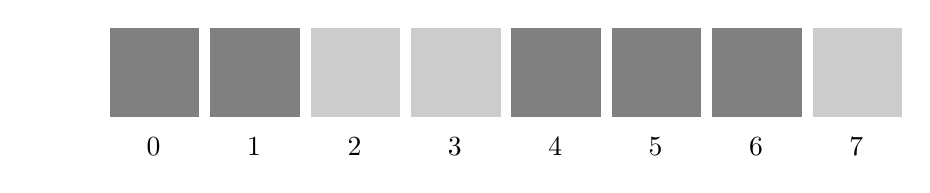
\begin{tikzpicture}[scale=.75]
\path (-1.4cm,0) -- (0,0);  % Space for robot
\foreach \n/\x/\color in
  {0/0/100, 1/1.7/100, 2/3.4/40, 3/5.1/40,
   4/6.8/100, 5/8.5/100, 6/10.2/100, 7/11.9/40} {
    \draw[fill,color=gray!\color] (\x,0) rectangle +(1.5,1.5);
    \node[xshift=.55cm] at (\x, -5mm) {\p{\n}};
}
\end{tikzpicture}
\end{center}

Pour plus de clarté, les portes et les murs sont dessinés comme s'ils se trouvaient sur le sol et que le robot se déplaçait au-dessus d'eux, en mesurant l'intensité à l'aide de capteurs au sol.

La tâche du robot consiste à franchir une porte spécifique, par exemple celle qui se trouve à la position 4. Mais comment le robot peut-il savoir où il se trouve ? Grâce à l'odométrie, le robot peut déterminer sa position actuelle à partir d'une position de départ connue. Par exemple, si le robot se trouve à l'extrémité gauche du mur :
\begin{center}
% Robot trying to localize 2
\begin{tikzpicture}[scale=.75]
\path (-1.4cm,0) -- (0,0);  % Space for robot
\foreach \n/\x/\color in
  {0/0/100, 1/1.7/100, 2/3.4/40, 3/5.1/40,
   4/6.8/100, 5/8.5/100, 6/10.2/100, 7/11.9/40} {
    \draw[fill,color=gray!\color] (\x,0) rectangle +(1.5,1.5);
    \node[xshift=.55cm] at (\x, -5mm) {\p{\n}};
}
\pic[scale=.5,fill] at (-1.1cm,7.5mm) { robot };
\end{tikzpicture}
\end{center}
il sait qu'il doit se déplacer de cinq fois la largeur de chaque porte, alors que si le robot se trouve à la position suivante :
\begin{center}
% Robot trying to localize 3
\begin{tikzpicture}[scale=.75]
\path (-1.4cm,0) -- (0,0);  % Space for robot
\foreach \n/\x/\color in
  {0/0/100, 1/1.7/100, 2/3.4/40, 3/5.1/40,
   4/6.8/100, 5/8.5/100, 6/10.2/100, 7/11.9/40} {
    \draw[fill,color=gray!\color] (\x,0) rectangle +(1.5,1.5);
    \node[xshift=.55cm] at (\x, -5mm) {\p{\n}};
}
\pic[scale=.5,fill] at (5.5cm,7.5mm) { robot };
\end{tikzpicture}
\end{center}
la porte souhaitée est la prochaine à droite. En raison des erreurs d'odométrie, il est fort probable que le robot se perde au fil du temps. Dans cette section, nous implémentons une version unidimensionnelle d'un algorithme probabiliste de localisation \emph{Markov}\index{algorithme de Markov} qui prend en compte l'incertitude dans les capteurs et dans le mouvement du robot, et renvoie les emplacements les plus probables du robot.

\ref{a.bayes} contient un bref tutoriel sur la probabilité conditionnelle et la règle de Bayes, y compris un exemple des détails des calculs de l'incertitude.

\subsection{La détection augmente la certitude}

Considérons un robot dans l'environnement ci-dessus, composé de murs et de portes, qui ne dispose d'aucune information sur son emplacement. Le robot attribue une probabilité aux huit positions où il pourrait se trouver. Au départ, il n'a aucune idée de l'endroit où il se trouve, et chaque position se verra donc attribuer la probabilité $b[i]=1.0/8=.125\approx .13$, où $b$ est appelé le \emph{réseau de croyance}:\footnote{Toutes les probabilités seront arrondies à deux chiffres décimaux pour l'affichage.}
\begin{center}
\begin{tikzpicture}
\draw (0,3) node[left] {\p{1.0}} -- node[left] {$p$} (0,0) node[left] {\p{0.0}} -- node[below,yshift=-4mm] {$b$} (8,0);
\foreach \n/\v in {0/.13, 1/.13, 2/.13, 3/.13, 4/.13, 5/.13, 6/.13, 7/.13}
  \pic { bar=\n/\v };
\foreach \n in {.5, 1.5, 4.5, 5.5, 6.5}
  \node at (\n,3) {$\bullet$};
\pic[scale=.2] at (4.4,2.5) { robot };
\end{tikzpicture}
\end{center}
Dans les graphiques, les points indiquent les positions des portes et une petite icône indique la position actuelle du robot, qui est orienté vers la droite.

Supposons maintenant que les capteurs du robot détectent une zone gris foncé. Son incertitude est réduite, car il sait qu'il doit se trouver devant l'une des cinq portes. Le tableau de croyances indique $.2$ pour chacune des portes et $.0$ pour chacun des murs :
\begin{center}
\begin{tikzpicture}
\draw (0,3) node[left] {\p{1.0}} -- node[left] {$p$} (0,0) node[left] {\p{0.0}} -- node[below,yshift=-4mm] {$b$} (8,0);
\foreach \n/\v in {0/.2, 1/.2, 2/.0, 3/.0, 4/.2, 5/.2, 6/.2, 7/.0}
  \pic { bar=\n/\v };
\foreach \n in {.5, 1.5, 4.5, 5.5, 6.5}
  \node at (\n,3) {$\bullet$};
\pic[scale=.2] at (4.4,2.5) { robot };
\end{tikzpicture}
\end{center}
Le robot se déplace ensuite vers l'avant et détecte à nouveau une zone gris foncé. Il n'y a plus que trois possibilités : il était à la position 0 et s'est déplacé vers 1, il était à 4 et s'est déplacé vers 5, ou il était à 5 et s'est déplacé vers 6. Si la position initiale du robot était 1 ou 6, après s'être déplacé vers la droite, il ne détecterait plus de zone gris foncé et ne pourrait donc pas s'y trouver. La probabilité est maintenant de $.33$ pour chacune des trois positions 1, 4, 5 :
\begin{center}
\begin{tikzpicture}
\draw (0,3) node[left] {\p{1.0}} -- node[left] {$p$} (0,0) node[left] {\p{0.0}} -- node[below,yshift=-4mm] {$b$} (8,0);
\foreach \n/\v in {0/.0, 1/.33, 2/.0, 3/.0, 4/.0, 5/.33, 6/.33, 7/.0}
  \pic { bar=\n/\v };
\foreach \n in {.5, 1.5, 4.5, 5.5, 6.5}
  \node at (\n,3) {$\bullet$};
\pic[scale=.2] at (5.4,2.5) { robot };
\end{tikzpicture}
\end{center}
Après l'étape suivante du robot, s'il détecte à nouveau une porte, il se trouve sans aucun doute à la position 6 :
\begin{center}
\begin{tikzpicture}
\draw (0,3) node[left] {\p{1.0}} -- node[left] {$p$} (0,0) node[left] {\p{0.0}} -- node[below,yshift=-4mm] {$b$} (8,0);
\foreach \n/\v in {0/.0, 1/.0, 2/.0, 3/.0, 4/.0, 5/.0, 6/1.0, 7/.0}
  \pic { bar=\n/\v };
\foreach \n in {.5, 1.5, 4.5, 5.5, 6.5}
  \node at (\n,3) {$\bullet$};
\pic[scale=.2] at (6.4,2.5) { robot };
\end{tikzpicture}
\end{center}
\noindent{}Si le robot n'a pas détecté de porte, il se trouve soit à la position 2, soit à la position 7 :
\begin{center}
\begin{tikzpicture}
\draw (0,3) node[left] {\p{1.0}} -- node[left] {$p$} (0,0) node[left] {\p{0.0}} -- node[below,yshift=-4mm] {$b$} (8,0);
\foreach \n/\v in {0/.0, 1/.0, 2/.5, 3/.0, 4/.0, 5/.0, 6/.0, 7/.5}
  \pic { bar=\n/\v };
\foreach \n in {.5, 1.5, 4.5, 5.5, 6.5}
  \node at (\n,3) {$\bullet$};
\end{tikzpicture}
\end{center}
Le robot maintient un tableau de croyances et intègre de nouvelles données lorsqu'il détecte la présence ou l'absence d'une porte. Au fil du temps, l'incertitude diminue : le robot sait avec plus de certitude où il se trouve réellement. Dans cet exemple, le robot finit par connaître avec certitude sa position devant la porte $6$ ou par réduire son incertitude à l'une des deux positions $2,7$.

\subsection{Incertitude dans la détection}

Les valeurs renvoyées par les capteurs du robot reflètent l'intensité de la lumière réfléchie par les couleurs grises des portes et des murs. Si la différence de couleur entre une porte gris foncé et un mur gris clair n'est pas très importante, le robot peut parfois détecter une porte gris foncé comme un mur gris clair, ou inversement. Cela peut être dû à des changements dans l'éclairage ambiant ou à des erreurs dans les capteurs eux-mêmes. Il s'ensuit que le robot ne peut pas faire la distinction entre les deux avec une certitude totale.

Nous modélisons cet aspect du monde en attribuant des probabilités à la détection. Si le robot détecte du gris foncé, nous spécifions que la probabilité est de $.9$ qu'il ait correctement détecté une porte et de $.1$ qu'il ait détecté par erreur un mur où se trouvait en fait une porte. Inversement, s'il détecte du gris clair, la probabilité est de $.9$ qu'il ait correctement détecté un mur et de $.1$ qu'il ait détecté par erreur une porte là où il y avait un mur.

Nous continuons à afficher les calculs sous forme de graphiques, mais vous trouverez peut-être plus facile de les suivre dans le tableau~\ref{tab.uncertain-sensing}. Chaque ligne représente le tableau de croyances du robot suivant l'action écrite dans la première colonne.

\begin{table}
\caption[Localisation avec incertitude de détection]{Localisation avec incertitude de détection, capteur=après multiplication par l'incertitude du capteur, norme=après normalisation, droite=après déplacement d'une position vers la droite}
\label{tab.uncertain-sensing}
\setlength{\tabcolsep}{6pt}
\begin{tabular}{l|rrrrrrrr}
\hline
position&\multicolumn{1}{c}{$0$}&\multicolumn{1}{c}{$1$}&\multicolumn{1}{c}{$2$}&\multicolumn{1}{c}{$3$}&\multicolumn{1}{c}{$4$}&\multicolumn{1}{c}{$5$}&\multicolumn{1}{c}{$6$}&\multicolumn{1}{c}{$7$}\\
porte?&\multicolumn{1}{c}{$\bullet$}&\multicolumn{1}{c}{$\bullet$}&&&\multicolumn{1}{c}{$\bullet$}&\multicolumn{1}{c}{$\bullet$}&\multicolumn{1}{c}{$\bullet$}&\\
\hline
initial &$0.13$ & $0.13$ & $0.13$ & $0.13$ & $0.13$ & $0.13$ & $0.13$ & $0.13$\\
capteur  &$0.11$ & $0.11$ & $0.01$ & $0.01$ & $0.11$ & $0.11$ & $0.11$ & $0.01$\\
norme    &$0.19$ & $0.19$ & $0.02$ & $0.02$ & $0.19$ & $0.19$ & $0.19$ & $0.02$\\
\hline
droite   &$0.02$ & $0.19$ & $0.19$ & $0.02$ & $0.02$ & $0.19$ & $0.19$ & $0.19$\\
capteur  &$0.02$ & $0.17$ & $0.02$ & $0.00$ & $0.02$ & $0.17$ & $0.17$ & $0.02$\\
norme    &$0.03$ & $0.29$ & $0.03$ & $0.00$ & $0.03$ & $0.29$ & $0.29$ & $0.03$\\
\hline
droite   &$0.03$ & $0.03$ & $0.29$ & $0.03$ & $0.00$ & $0.03$ & $0.29$ & $0.29$\\
capteur  &$0.03$ & $0.03$ & $0.03$ & $0.00$ & $0.00$ & $0.03$ & $0.26$ & $0.03$\\
norme    &$0.07$ & $0.07$ & $0.07$ & $0.01$ & $0.01$ & $0.07$ & $0.63$ & $0.07$\\
\hline
\end{tabular}
\end{table}
Initialement, après avoir détecté un gris foncé à un endroit où se trouve une porte, nous savons avec une probabilité de $0,125 \times 0,9 = 0,1125$ qu'une porte a été correctement détectée ; cependant, il existe toujours une probabilité de $0,125 \times 0,1 = 0,0125$ qu'un mur ait été détecté par erreur. Après normalisation (\ref{a.normalize}), le tableau de croyances est le suivant :
\begin{center}
\begin{tikzpicture}
\draw (0,3) node[left] {\p{1.0}} -- node[left] {$p$} (0,0) node[left] {\p{0.0}} -- node[below,yshift=-4mm] {$b$} (8,0);
\foreach \n/\v in {0/.19, 1/.19, 2/.02, 3/.02, 4/.19, 5/.19, 6/.19, 7/.02}
  \pic { bar=\n/\v };
\foreach \n in {.5, 1.5, 4.5, 5.5, 6.5}
  \node at (\n,3) {$\bullet$};
\pic[scale=.2] at (4.4,2.5) { robot };
\end{tikzpicture}
\end{center}
Que se passe-t-il lorsque le robot se déplace d'une position vers la droite ? Son tableau de croyances doit également se déplacer d'une position vers la droite. Par exemple, la probabilité $.19$ que le robot était à la position $1$ devient la probabilité qu'il est à la position $2$. De même, la probabilité $.02$ que le robot soit à la position $3$ devient la probabilité qu'il soit à la position $4$. La probabilité que le robot soit à la position $0$ est maintenant de $0$ et la probabilité $b_7$ devient $b_8$, de sorte que les indices deviennent $1$--$8$ au lieu de $0$--$7$. Pour simplifier les calculs et les diagrammes de l'exemple, les indices $0$--$7$ sont conservés et la valeur de $b_8$ est stockée dans $b_0$ comme si la carte était cyclique. Le tableau de croyances après le déplacement du robot vers la droite est le suivant :
\begin{center}
\begin{tikzpicture}
\draw (0,3) node[left] {\p{1.0}} -- node[left] {$p$} (0,0) node[left] {\p{0.0}} -- node[below,yshift=-4mm] {$b$} (8,0);
\foreach \n/\v in {0/.02, 1/.19, 2/.19, 3/.02, 4/.02, 5/.19, 6/.19, 7/.19}
  \pic { bar=\n/\v };
\foreach \n in {.5, 1.5, 4.5, 5.5, 6.5}
  \node at (\n,3) {$\bullet$};
\pic[scale=.2] at (5.4,2.5) { robot };
\end{tikzpicture}
\end{center}
Si le robot détecte à nouveau du gris foncé, la probabilité de se trouver aux positions 1, 5 ou 6 devrait augmenter. Le calcul des probabilités et la normalisation donnent :
\begin{center}
\begin{tikzpicture}
\draw (0,3) node[left] {\p{1.0}} -- node[left] {$p$} (0,0) node[left] {\p{0.0}} -- node[below,yshift=-4mm] {$b$} (8,0);
\foreach \n/\v in {0/.03, 1/.29, 2/.03, 3/.0, 4/.03, 5/.29, 6/.29, 7/.03}
  \pic { bar=\n/\v };
\foreach \n in {.5, 1.5, 4.5, 5.5, 6.5}
  \node at (\n,3) {$\bullet$};
\pic[scale=.2] at (5.4,2.5) { robot };
\end{tikzpicture}
\end{center}
Le robot se déplace à nouveau vers la droite :
\begin{center}
\begin{tikzpicture}
\draw (0,3) node[left] {\p{1.0}} -- node[left] {$p$} (0,0) node[left] {\p{0.0}} -- node[below,yshift=-4mm] {$b$} (8,0);
\foreach \n/\v in {0/.03, 1/.03, 2/.29, 3/.03, 4/.0, 5/.03, 6/.29, 7/.29}
  \pic { bar=\n/\v };
\foreach \n in {.5, 1.5, 4.5, 5.5, 6.5}
  \node at (\n,3) {$\bullet$};
\pic[scale=.2] at (6.4,2.5) { robot };
\end{tikzpicture}
\end{center}
\noindent{}and senses a third dark gray area. The belief array becomes:
\begin{center}
\begin{tikzpicture}
\draw (0,3) node[left] {\p{1.0}} -- node[left] {$p$} (0,0) node[left] {\p{0.0}} -- node[below,yshift=-4mm] {$b$} (8,0);
\foreach \n/\v in {0/.07, 1/.07, 2/.07, 3/.01, 4/.0, 5/.07, 6/.63, 7/.07}
  \pic { bar=\n/\v };
\foreach \n in {.5, 1.5, 4.5, 5.5, 6.5}
  \node at (\n,3) {$\bullet$};
\pic[scale=.2] at (6.4,2.5) { robot };
\end{tikzpicture}
\end{center}
Il n'est pas surprenant que le robot se trouve presque certainement à la position 6.

\begin{framed}
\act{Localisation avec incertitude dans les capteurs}{local-uncertain}
\begin{itemize}
\item Mettre en œuvre la localisation probabiliste avec l'incertitude dans le capteur.
\item Comment le comportement de l'algorithme change-t-il lorsque l'incertitude est modifiée ?
\item Exécuter l'algorithme pour différentes positions de départ du robot.
\end{itemize}
\end{framed}

\section{Incertitude du mouvement}\label{s.uncertain-motion}

Outre l'incertitude liée aux capteurs, les robots sont soumis à l'incertitude liée à leur mouvement. Nous pouvons demander au robot de se déplacer d'une position vers la droite, mais il se peut qu'il se déplace de deux positions, ou qu'il se déplace très peu et reste dans sa position actuelle. Modifions l'algorithme pour prendre en compte cette incertitude.

Soit $b$ le tableau de croyances. Le tableau de croyances est mis à jour à l'aide de la formule suivante:
\begin{displaymath}
b'_i = p_i \, b_i\,,
\end{displaymath}
où $b'_i$ est la nouvelle valeur de $b_i$ et $p_i$ est la probabilité de détecter une porte (dans l'exemple, $p_i$ est $0,9$ pour $i=0,1,4,5,6$ et $p_i$ est $0,1$ pour $i=2,3,7$). Si le mouvement est certain, le robot se déplace d'une position vers la droite, mais avec un mouvement incertain, le calcul suivant prend en compte les probabilités $q_j$ que le robot se déplace effectivement de $j=0,1,2$ positions :
\begin{displaymath}
b'_i = p_i \,(b_{i-2}\, q_2 + b_{i-1}\, q_1 + b_{i}\, q_0)\,,
\end{displaymath}
comme le montre le diagramme suivant :
\begin{center}
\begin{tikzpicture}[scale=1.1]
\begin{scope}[every node/.style={draw,rectangle,minimum size=1cm}]
\node (b2)  {$b_{i-2}$};
\node (b1)  [right=of b2] {$b_{i-1}$};
\node (b)   [right=of b1] {$b_{i}$};
\node (b2p) [below=of b2] {};
\node (b1p) [below=of b1] {};
\node (bp)  [below=of b]  {$b'$};
\end{scope}
\draw[->] (b2.south) -- node[below,near start] {$q_2$} (bp.north west);
\draw[->] (b1.south) -- node[above] {$q_1$} (bp.north);
\draw[->] (b.south)  -- node[above,near end,xshift=6pt] {$q_0$} (bp.north east);
\end{tikzpicture}
\end{center}
It is highly likely that the robot will move correctly, so reasonable values are $q_1=0.8$ and $q_0=q_2=0.1$. With these values for the uncertainty of the motion and the previous values for $p_i$, the calculation of the belief array after three moves is shown in Table~\ref{tab.uncertain-sensing-motion} and its final value is shown in the following diagram:
\begin{center}
\begin{tikzpicture}
\draw (0,3) node[left] {\p{1.0}} -- node[left] {$p$} (0,0) node[left] {\p{0.0}} -- node[below,yshift=-4mm] {$b$} (8,0);
\foreach \n/\v in {0/.11, 1/.21, 2/.05, 3/.01, 4/.02, 5/.13, 6/.43, 7/.05}
  \pic { bar=\n/\v };
\foreach \n in {.5, 1.5, 4.5, 5.5, 6.5}
  \node at (\n,3) {$\bullet$};
\pic[scale=.2] at (1.4,2.5) { robot };
\node at (2,2.5) {\p{?}};
\pic[scale=.2] at (6.4,2.5) { robot };
\node at (7,2.5) {\p{?}};
\end{tikzpicture}
\end{center}
Le robot est probablement en position 6, mais nous sommes moins sûrs car la probabilité n'est que de $.43$ au lieu de $.63$. Il y a une probabilité non négligeable de $.21$ que le robot soit en position 1.

\begin{table}
\caption[Localisation avec incertitude de détection et de mouvement]{Localisation avec incertitude de détection et de mouvement, capteur=après multiplication par l'incertitude du capteur, norme=après normalisation, droite=après déplacement d'une position vers la droite}\label{tab.uncertain-sensing-motion}
\setlength{\tabcolsep}{6pt}
\begin{tabular}{l|rrrrrrrr}
\hline
position&\multicolumn{1}{c}{$0$}&\multicolumn{1}{c}{$1$}&\multicolumn{1}{c}{$2$}&\multicolumn{1}{c}{$3$}&\multicolumn{1}{c}{$4$}&\multicolumn{1}{c}{$5$}&\multicolumn{1}{c}{$6$}&\multicolumn{1}{c}{$7$}\\
porte?&\multicolumn{1}{c}{$\bullet$}&\multicolumn{1}{c}{$\bullet$}&&&\multicolumn{1}{c}{$\bullet$}&\multicolumn{1}{c}{$\bullet$}&\multicolumn{1}{c}{$\bullet$}&\\
\hline
initial  & $0.13$ & $0.13$ & $0.13$ & $0.13$ & $0.13$ & $0.13$ & $0.13$ & $0.13$\\
capteur & $0.11$ & $0.11$ & $0.01$ & $0.01$ & $0.11$ & $0.11$ & $0.11$ & $0.01$\\
norme     & $0.19$ & $0.19$ & $0.02$ & $0.02$ & $0.19$ & $0.19$ & $0.19$ & $0.02$\\
\hline
droite    & $0.05$ & $0.17$ & $0.17$ & $0.04$ & $0.04$ & $0.17$ & $0.19$ & $0.17$\\
capteur & $0.05$ & $0.17$ & $0.02$ & $0.00$ & $0.03$ & $0.15$ & $0.17$ & $0.02$\\
norme     & $0.08$ & $0.27$ & $0.03$ & $0.01$ & $0.06$ & $0.25$ & $0.28$ & $0.03$\\
\hline
droite    & $0.06$ & $0.09$ & $0.23$ & $0.05$ & $0.01$ & $0.07$ & $0.23$ & $0.25$\\
capteur & $0.05$ & $0.10$ & $0.02$ & $0.01$ & $0.01$ & $0.06$ & $0.21$ & $0.02$\\
norme     & $0.11$ & $0.21$ & $0.05$ & $0.01$ & $0.02$ & $0.13$ & $0.43$ & $0.05$\\
\hline
\end{tabular}
\end{table}

\begin{framed}
\act{Localisation avec incertitude dans le mouvement}{local-motion}
\begin{itemize}
\item Mettre en œuvre la localisation probabiliste avec incertitude dans le calcul de la puissance du moteur.
\item Comment le comportement de l'algorithme change-t-il lorsque l'incertitude est modifiée ?
\item Exécuter l'algorithme pour différentes positions de départ du robot.
\end{itemize}
\end{framed}

\section{Résumé}

L'odométrie fournit une estimation de la position d'un robot. Un robot peut utiliser des techniques d'arpentage pour calculer sa position par rapport à un objet dont la position est connue. Le GPS fournit d'excellentes données sur la localisation, mais il n'est pas toujours assez précis et les interférences avec la réception des satellites limitent son utilisation dans les environnements intérieurs. Si le robot peut détecter plusieurs objets connus et s'il dispose d'une carte de son environnement, il peut utiliser la localisation probabiliste pour estimer sa position avec une probabilité élevée, bien que cette probabilité soit réduite si les capteurs ou les mouvements du robot sont très incertains.

\section{Lecture complémentaire}

Les méthodes probabilistes en robotique sont traitées en profondeur dans \cite{thrun}. Le site \url{http://www.gps.gov} contient une mine d'informations sur le GPS. Une mise en œuvre de la localisation probabiliste à l'aide du robot éducatif Thymio est décrite dans \cite{wang2016dars}.
